\documentclass[12pt, a4paper]{scrartcl}

% CONFIG
\newcommand{\exptitle}{Lange Halbwertszeiten}      % long name of experiment 
\newcommand{\exptitleshort}{LHWZ} % short name of experiment
\newcommand{\expdate}{8. September 2014}             % date of experiment

% PACKAGES + MODIFICATIONS
\usepackage[ngerman]{babel} %standard language stuff
\usepackage[T1]{fontenc}
\usepackage[utf8]{inputenc}

\usepackage[fleqn]{amsmath}  % math
\usepackage{amssymb}

\usepackage{graphicx} %graphics
\usepackage{float} 

\usepackage[automark,headsepline]{scrlayer-scrpage} %headings
\pagestyle{scrheadings}
\ihead{\exptitleshort}
\ohead{\pagemark}
\cfoot{}

\usepackage{hyperref}
\hypersetup{
    unicode=true,          % non-Latin characters in Acrobat’s bookmarks
    pdftoolbar=true,       % show Acrobat’s toolbar?
    pdfmenubar=true,       % show Acrobat’s menu?
    pdffitwindow=false,    % window fit to page when opened
    pdfstartview={FitH},   % fits the width of the page to the window
    pdfnewwindow=true,     % links in new window
    colorlinks=true,       % false: boxed links; true: colored links
    linkcolor=black,       % color of internal links (change box color with linkbordercolor)
    citecolor=green,       % color of links to bibliography
    filecolor=magenta,     % color of file links
    urlcolor=cyan          % color of external links
}

\usepackage{chngcntr}
\counterwithin{figure}{section}  % number figures per section
\numberwithin{equation}{section} % number equations per section

\usepackage{enumerate} % better way to config enumerates

\setcounter{tocdepth}{2} % table of contents depth

\setlength{\parindent}{0pt} % no indent on new paragraph

% NEW COMMANDS
\newcommand{\chemel}[2]{\texorpdfstring{${}^{#2}\text{#1}$ }{#1-#2}}
\newcommand{\uran}{\chemel{U}{238}}
\newcommand{\samarium}{\chemel{Sm}{147}}
\newcommand{\kalium}{\chemel{K}{40}}

% DOCUMENT SETTINGS

\title{\exptitle}
\subtitle{Fortgeschrittenen-Praktikum 1}
\author{Moritz Bitterling und Benjamin Rottler \\ Universität Freiburg}
\date{\expdate}
\publishers{\vspace{3cm} \includegraphics[height=8cm]{../../img/logo_uni.pdf}}
%TODO links unten Name von Betreuer einfügen

% DOCUMENT
\begin{document}

\hypersetup{pageanchor=false} %stop page numbering (hyperref) to prevent for double page numers
\maketitle
\thispagestyle{empty}

\newpage
\tableofcontents
\thispagestyle{empty}

\newpage
\hypersetup{pageanchor=true} %start page numbering again
\setcounter{page}{1} %set to page 1

\section{Versuchsziel}
Im Halbleiter-Versuch werden in drei verschieden Versuchsteilen unterschiedliche
halbleiterphysikalische Effekte untersucht:
Mit einer Transmissions- und Absorptionsmessung werden die \emph{Bandlücken} von Germanium und Silizium bestimmt.
Beim Haynes-Shockley-Experiment erhält man Informationen über die \emph{Mobilität}, \emph{Diffusionskonstante} und
\emph{mittlere Lebensdauer} der Elektronen im Leitungsband von Germanium.
Außerdem wird mit dotierten Halbleitern das \emph{Energiespektrum} von radioaktiven Proben aufgenommen. 
\section{Physical Principles}
\subsection{Born-Oppenheimer approximation}
Since molecules have a much more complicated Hamiltonian than a hydrogen atom, it is not possible to solve the Schrödinger equation analytical. 
A good approximation for this problem is the \emph{Born-Oppenheimer approximation}.  \\
The reasoning is in the following way: The nuclei are much heavier than the electrons of the molecule ($m_{\text{nucleus}} >> m_{\text{electron}}$). 
Thus the electrons live in a much shorter time scale than the nuclei. They react almost immediately to 
changes of the nuclei and are only minimally affected by the proper motion of the nuclei. According to the \emph{Born-Oppenheimer approximation} 
you can write the whole wave function as a product of the wave functions of the nuclei and the electrons:
\begin{equation}
\label{eq:boapprox}
  \Psi_{\text{total}} = \Psi_{\text{electrons}} \cdot \Psi_{\text{nuclei}}
\end{equation}

\subsection{Energy levels of oscillation}
In a two atomic molecule the two nuclei interact with each other in a mutual potential $V$. In analogy to the two-body problem in classical 
mechanics you can reduce the problem to a problem with only one particle with a reduced mass $\mu = \frac{m_1 m_2}{m_1 + m_2}$ and an effective 
potential $V(r)$. The Schrödinger equation is 
\begin{equation}
\label{eq_schroedinger}
  \left( - \frac{\hbar^2}{2 \mu} \frac{\difd^2}{\difd r^2} + V(r) \right) \Psi(r) = E \Psi(r) .
\end{equation}
For small oscillations around the minimum $r_e$ you can perform a series expansion on the potential $V(r)$:
\begin{equation}
\begin{split}
\label{eq_potential_series}
  V(r) = &  V(r_e) + \underbrace{\left. \frac{\partial V(r)}{\partial r} \right|_{r=r_e}}_{=0} (r-r_e)
     + \left. \frac{1}{2} \frac{\partial^2 V(r)}{\partial r^2} \right|_{r=r_e}(r-r_e)^2 \\
  & + \left. \frac{1}{6} \frac{\partial^3 V(r)}{\partial r^3} \right|_{r=r_e}(r-r_e)^3 + \ldots \\
  = & V(r_e) + \frac{1}{2} V''(r_e)(r-r_e)^2 + \frac{1}{6} V'''(r_e)(r_re)^3 + \ldots
\end{split}
\end{equation}
If you approximate the potential only up to second order the potential equals the potential of a harmonic oscillator with known frequencies and 
eigenenergies:
\begin{equation}
\label{eq:ho:freq}
  \omega = \sqrt{\frac{V''(r_e)}{m}}
\end{equation}
\begin{equation}
\label{eq:ho:energy}
  E(\nu) =  \hbar \omega \left( \nu + \frac{1}{2} \right), \qquad \nu = 0, 1, 2, \ldots
\end{equation}
For higher energy levels this approximation is not good enough and you need to consider higher orders of the series expansion. You can solve the
Schrödinger equation with perturbation theory and it yields the eigenenergies of an inharmonic oscillator:
\begin{equation}
\label{eq:iho:energy}
  G(\nu) = \omega_e \left( \nu + \frac{1}{2} \right) - \omega_e x_e \left( \nu + \frac{1}{2} \right)^2 
            + \omega_e y_e \left( \nu + \frac{1}{2} \right)^3 + \ldots, \qquad \nu = 0, 1, 2, \ldots
\end{equation}
The factor $\omega_e$ corresponds to the oscillation frequency of the harmonic oscillator, the factors $\omega_e x_e$, $\omega_e y_e, \ldots$ 
describe the inharmonicity of the potential. \\
The difference between two adjacent eigenenergies is
\begin{equation}
\label{eq:iho:energydiff}
  \Delta G \left( \nu + \frac{1}{2} \right) = G(\nu + 1) - G(\nu) = \omega_e - \omega_e x_e (2\nu + 2) + \omega_e y_e \left( 3\nu^2 + 6 \nu + \frac{13}{4} \right) + \ldots 
\end{equation}
Provided that $\omega_e x_e$ is positive (and it is for the $I_2$-molecule) there is an 
$\nu_{\text{diss}}$ with $\Delta G (\nu_{\text{diss}} + \frac{1}{2}) = 0$. If the energy of the molecule is above this energy level it 
is dissociated, the atoms split into two ions. \\
The dissociation energy from the lowest energy level is
\begin{equation}
\label{eq:dissenergy}
  D_0 = \sum_{\nu=0}^{\nu_{\text{diss}}} \Delta G \left( \nu + \frac{1}{2} \right),
\end{equation}
and from the minimum of the potential
\begin{equation}
\label{eq:dissenergy2}
  D_e = G(0) + D_0
\end{equation} 
Since $\hbar \omega = h f$, $f = \frac{c}{\lambda}$ and $\lambda = \frac{1}{\bar{\nu}}$ the energy of vibrational states often is denoted in 
wavenumbers $\bar{\nu}$ (in multiples of $h c$, because $E = hc\bar{\nu}$) with the dimension $\text{cm}^{-1}$.

\subsection{Morse potential}
A good approximation of the real potential of a two atomic molecule is the \emph{Morse potential}
\begin{equation}
  V(r) = D_e \left( 1 - e^{-a(r-r_e)} \right)^2
\end{equation}
with dissociation energy (from minimum of potential) $D_e$ , a molecule specific constant $a$  and the internuclear distance $r_e$. \\
The Schrödinger equation for this potential yields for the constants in \autoref{eq:iho:energy}:
\begin{equation}
\label{eq:morse_we}
  w_e = a \sqrt{\frac{\hbar D_e}{\pi c \mu}}
\end{equation}
\begin{equation}
\label{eq_morse_wexe}
  w_e x_e = \frac{\hbar a^2}{2 \omega_e x_e}
\end{equation}
The Dissociation energy can be calculated with those two constants:
\begin{equation}
\label{eq:morse_dissenergy}
  D_e = \frac{\omega_e^2}{4 \omega_e x_e}
\end{equation}

\subsection{Absorption of radiation}
-Frank-Condon principle \\
-progression

\subsection{Rotation}
-formula with rotational constant

\subsection{Statistics}
\subsubsection{Weighted mean}
Different values $x_i$ with individual errors $s_i$ are given. The weighted (arithmetic) mean and its error is:
\begin{equation}
\label{eq:meanw}
  \bar{x} = \frac{\sum_i \frac{x_i}{s_i^2}}{\sum_i \frac{1}{s_i^2}}, \qquad s_{\bar{x}}^2 = \frac{1}{\sum_i \frac{1}{s_i^2}}
\end{equation}
\section{Versuchsaufbau}

\begin{figure}[H]
\begin{center}
  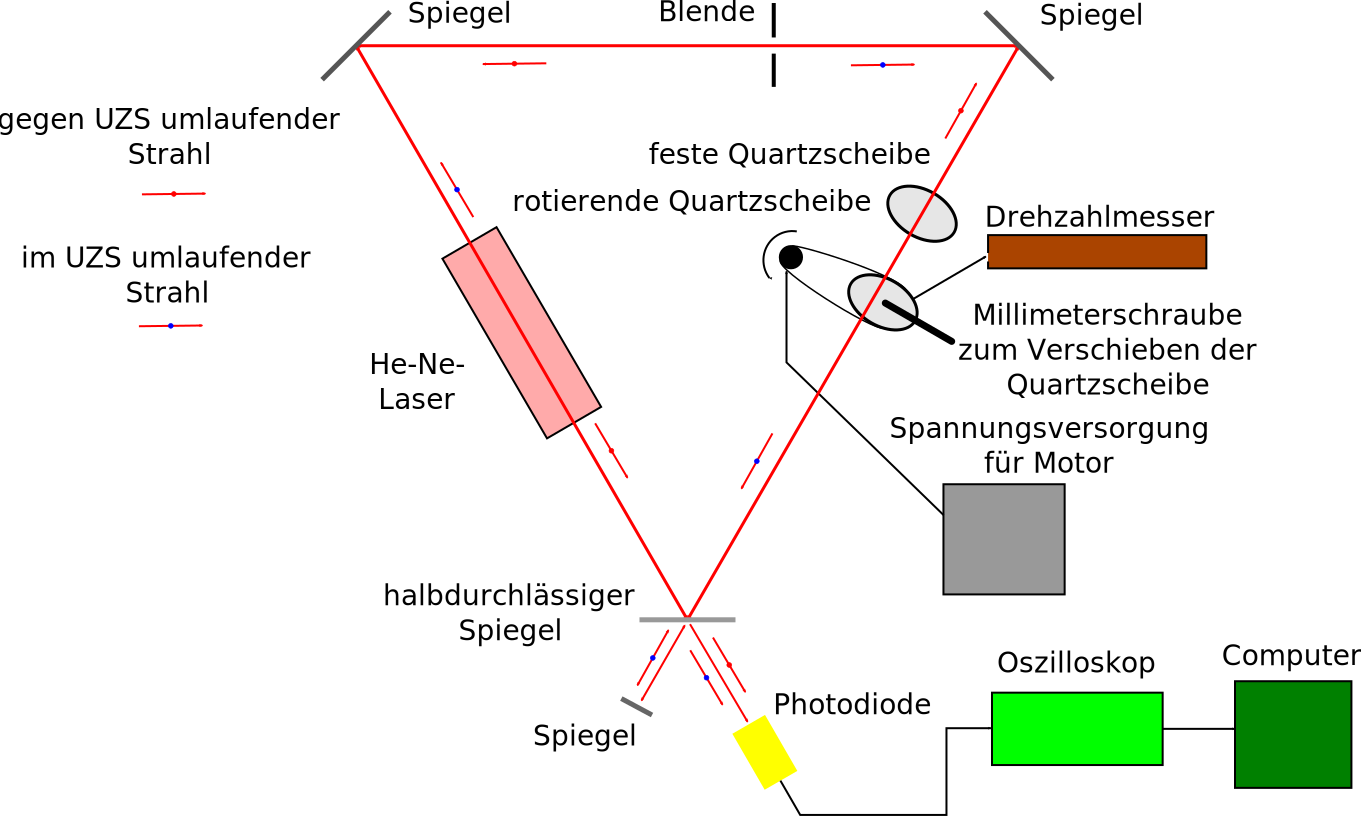
\includegraphics[width=0.95\textwidth]{../img/aufbau.pdf}
  \caption{Aufbau zur Bestimmung des Mitführungskoeffizinenten von Quarz mit einem Ringlaser.}
  \label{img:aufbau}
\end{center}
\end{figure}
\autoref{img:aufbau} zeigt den Aufbau des Ringlasers,
mit dem die Messungen durchgeführt werden.
Um eine Helium-Neon-Röhre,
die von einem statischen elektrischen Feld gepumpt wird,
ist mit drei Spiegeln ein Resonator aufgebaut.
Einer der Spiegel ist halbdurchlässig, um den Laserstrahl auszukoppeln.
Ein vierter Spiegel reflektiert den im Uhrzeigersinn umlaufenden Stahl so,
dass er zusammen mit dem anderen auf eine Photodiode fällt.
Der vierte Spiegel und der Halbdurchlässige können in ihrer Position verändert werden.
Im Strahlengang befindet sich außerdem eine einstellbare Blende,
mit der der Strahl abgeschwächt werden kann.
Zusätzlich sind im Strahlengang zwei Quarzscheiben,
die im Brewsterwinkel vom Laserstrahl getroffen werden.
Eine davon kann mit einem Motor in Rotation versetzt und ihre Drehzahl gemessen werden.
Die zweite, ruhende Scheibe ist dazu da,
den abgelenkten Strahl wieder zurück in den ursprünglichen Strahlverlauf zu brechen.\\
Das Signal der Photodiode wird auf einem Oszilloskop angezeigt und kann
vom Computer ausgelesen werden.
\section{Versuchsdurchführung}

\subsection{Kalibrierung des Aufbaus}
\label{sub:calibration}

Vor Durchführung der Messungen wird die Winkeleinstellung des Polarisators kalibriert
und der Strom der Helmholtz-Spulen so eingestellt,
dass Störmagnetfelder in z-Richtung kompensiert werden.

Das Kalibrierungskriterium für die Winkeleinstellungen ('0$^\circ$'-Position und '90$^\circ$'-Position)
ist die Symmetrie des Hanle-Signals und die Differenz zwischen
der Höhe des rechts- und des linksseitigen Untergrundes.
Die Lage der beiden Einstellungen wird grob abgeschätzt (um -20$^\circ$ und um 70$^\circ$)
und dann in 2$^\circ$-Schritten die Hanle-Signale aufgezeichnet.
\autoref{img:durchf:winkel} zeigt zwei der gemessenen
Signale. Auf der ersten Abbildung ist die Asymmetrie deutlich zu erkennen,
auf der zweiten Abbildung ist das Signal fast symmetrisch.
Folgende Winkel wurden für '0$^\circ$'-, '45$^\circ$'- und '90$^\circ$'-Position gewählt:
\begin{equation}
\label{eq:calang}
 \varphi_0=\text{-}18^\circ, \qquad \varphi_{45}=21^\circ, \qquad \varphi_{90}=66^\circ
\end{equation}
\begin{figure}[H]
\begin{center}
  \includegraphics[width=0.49\textwidth]{../data/1/-7_5.png}
  \includegraphics[width=0.49\textwidth]{../data/1/-20.png}
  \caption{Asymmetrisches Hanle-Signal bei $\varphi=\text{-}8^\circ$ (links) und
  annähernd symmetrisches Signal bei $\varphi=\text{-}20^\circ$ (rechts).}
  \label{img:durchf:winkel}
\end{center}
\end{figure}
Der Kompensationsstrom der Spulen wird eingestellt, indem die Breite des Hanle-Signals und
(in der 90$^\circ$-Position) die Signalintensität minimiert werden.
Es wird ebenfalls zuerst die korrekte Einstellung grob abgeschätzt (um -250\,mA)
und dann das Signal für mehrere Einstellungen aufgezeichnet.
Zwei Signale sind auf \autoref{img:durchf:strom} gezeigt:
Für $I_z$=400\,mA ist das Signal deutlich breiter als für $I_z$=175\,mA.
Als Kompensationsstrom wurden 
\begin{equation}
\label{eq:calcurr}
 I_z=280\,\text{mA} \qquad \text{und} \qquad I_y=0\,\text{mA}
\end{equation}
gewählt. (In y-Richtung wurde keine Kompensation durchgeführt,
da hier keine Abhängigkeit der Messergebnisse besteht.)
\begin{figure}[H]
\begin{center}
  \includegraphics[width=0.49\textwidth]{../data/2/-17_5X-40.png}
    \includegraphics[width=0.49\textwidth]{../data/2/-17_5X-27_5.png}
  \caption{Breites Hanle-Signal bei $I_z=$ -400\,mA (links) und schmales Signal bei $I_z$= -275\,mA (rechts).}
  \label{img:durchf:strom}
\end{center}
\end{figure}



\subsection{Messung des Hanle-Signals}

Für die Messung des Hanle-Signals wird die Temperatur am Aufbau schrittweise abgesenkt.
Am Netzteil des Peltierelements wird dazu eine Spannung eingestellt, nach 30 Minuten Abkühlzeit
die gemessene Temperatur notiert und Messungen mit den drei oben gewählten Winkeleinstellungen durchgeführt.



\section{Messergebnisse und Auswertung}

\subsection{Teil I: Pockels-Effekt}

\subsubsection{Sägezahnmethode}

\begin{figure}[H]
\begin{center}
  \includegraphics[width=15cm]{../img/pock_saege_winkel0.pdf}
  \caption{Deformiertes Photodiodensignal (blau) bei Einstellung der Achse des Analysators in
  Richtung höchster Transmission der Pockelszelle.}
  \label{img:pock_saege_winkel0}
\end{center}
\end{figure}

\autoref{img:pock_saege_winkel0} zeigt das Photodiodensignal, wenn der Analysator so eingestellt wird,
wie in der Versuchsanleitung beschrieben, so dass die Amplitude des Photodiodensignals maximiert wird.
Diese Einstellung ist zum Ablesen von Maximum und Minimum des Signals nicht geeignet.
\autoref{img:pock_saege_winkel1}, \autoref{img:pock_saege_winkel2} und \autoref{img:pock_saege_winkel3}
zeigen Messungen mit niedrigerer Amplitude, die für die Auswertung verwendet wurden.
In \autoref{tab:minmax} sind die Positionen von Maximum und Minimum für die drei Messungen aufgeführt.
Diese Positionen wurden durch Fits von Parabeln (mit den Fitparametern $a$, $b$ und $s$) an die Messdaten gewonnen:
\begin{equation}
  y = a \cdot (x-s)^2+b
\end{equation}
$s$ ist die Position des Minimums auf der x-Achse.\\
Die Steigung der Sägezahnfunktion wird mit einem Steigungsdreieck abgeschätzt:
Mit den Werten am Einsatzpunkt und am höchsten Punkt der Spannung erhält man folgende Steigung:
\begin{equation}
  m_s = \frac{U_2-U_1}{t_2-t_1} = 50 \,\frac{\text{V}}{\text{s}}
\end{equation}

\begin{figure}[H]
\begin{center}
  \includegraphics[width=15cm]{../img/pock_saege_winkel1.pdf}
  \caption{capt.}
  \label{img:pock_saege_winkel1}
\end{center}
\end{figure}

\begin{figure}[H]
\begin{center}
  \includegraphics[width=15cm]{../img/pock_saege_winkel2.pdf}
  \caption{capt.}
  \label{img:pock_saege_winkel2}
\end{center}
\end{figure}

\begin{figure}[H]
\begin{center}
  \includegraphics[width=15cm]{../img/pock_saege_winkel3.pdf}
  \caption{capt.}
  \label{img:pock_saege_winkel3}
\end{center}
\end{figure}

\subsubsection{Modulierte Gleichspannung}

\subsection{Teil II: Faraday-Effekt}
\section{Zusammenfassung und Diskussion}

Zusammenfassung der Messergebnisse, Vergleich mit Literaturwerten.

\end{document}